\documentclass[tikz,border=8pt]{standalone}
% Shared look for every TikZ diagram. Load with \input{../../tools/tikz-style.tex}
\usepackage[sfdefault]{roboto}
\usetikzlibrary{arrows.meta, positioning, shapes.geometric, calc, fit, backgrounds}
\definecolor{cblue}{HTML}{4C78A8}
\definecolor{corange}{HTML}{F58518}
\definecolor{cgreen}{HTML}{54A24B}
\definecolor{cred}{HTML}{E45756}
\definecolor{cpurple}{HTML}{B279A2}
\definecolor{cgrey}{HTML}{6B6B6B}
\tikzset{
  every picture/.style={font=\sffamily, line width=1.2pt},
  box/.style={draw=#1, fill=#1!12, rounded corners=4pt, align=center, inner sep=7pt, minimum height=1.1cm},
  box/.default=cgrey,
  arrow/.style={-{Stealth[length=3mm]}, draw=cgrey, line width=1.4pt},
  title/.style={font=\sffamily\bfseries\Large},
  note/.style={font=\sffamily\small, text=cgrey, align=center},
}
\AtBeginDocument{\hyphenpenalty=10000 \exhyphenpenalty=10000}

% The landmark bound at B in the town (roadkit: fastest travel times by Dijkstra). Fastest B to L: 193.8 s;
% fastest T to L: 46.8 s; true fastest B to T: 156.0 s. Going B -> T -> L is one way from B to L, so it is never
% faster than the fastest: 156.0 + 46.8 = 202.8 >= 193.8; hence B to T is at least 193.8 - 46.8 = 147.0 s.
\begin{document}
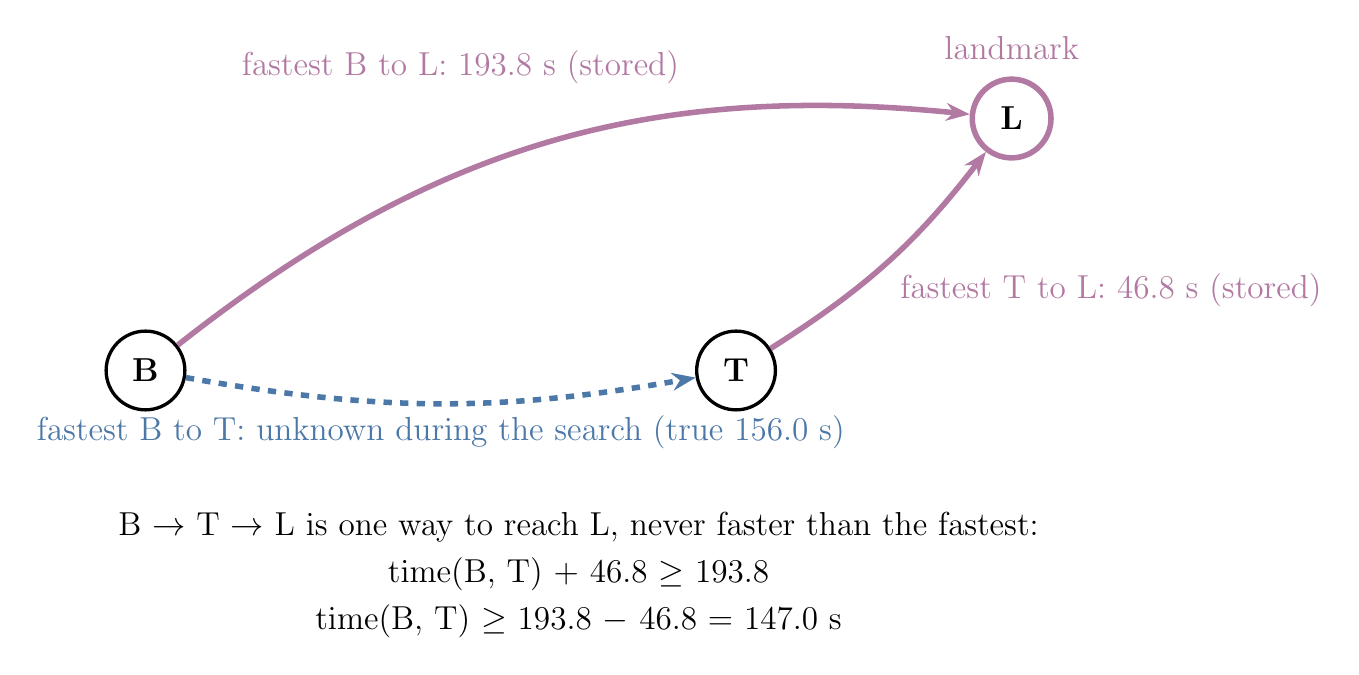
\begin{tikzpicture}[every node/.append style={font=\large},
  pt/.style={circle, draw=black, fill=white, minimum size=1.0cm, inner sep=0pt, font=\large\bfseries}]
  \node[pt] (B) at (0,0) {B};
  \node[pt] (T) at (7.5,0) {T};
  \node[pt, draw=cpurple, line width=2pt] (L) at (11,3.2) {L};
  \node[cpurple, above=2pt of L] {landmark};
  \draw[arrow, cpurple, line width=2pt] (B) to[bend left=22] (L);
  \node[text=cpurple] at (4.0,3.85) {fastest B to L: 193.8 s (stored)};
  \draw[arrow, cpurple, line width=2pt] (T) to[bend right=10] node[below right, text=cpurple] {fastest T to L: 46.8 s (stored)} (L);
  \draw[arrow, cblue, line width=2pt, dashed] (B) to[bend right=10] node[below, text=cblue] {fastest B to T: unknown during the search (true 156.0 s)} (T);
  \node[align=center, font=\large] at (5.5,-2.6) {B $\rightarrow$ T $\rightarrow$ L is one way to reach L, never faster than the fastest:\\[3pt]
     time(B, T) $+$ 46.8 $\ge$ 193.8\\[3pt]
     time(B, T) $\ge$ 193.8 $-$ 46.8 $=$ 147.0 s};
\end{tikzpicture}
\end{document}
